\documentclass[tikz]{standalone}
\begin{document}
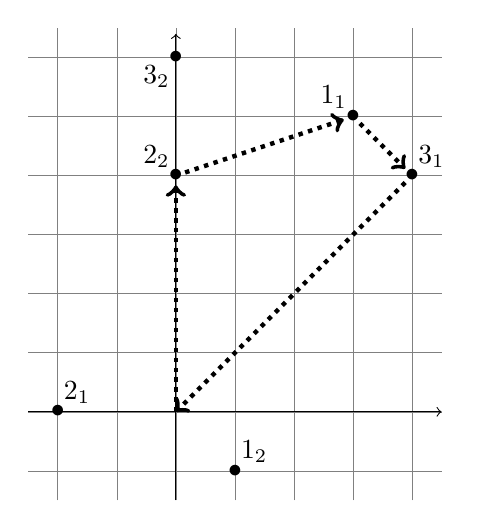
\begin{tikzpicture}[scale = .75, every node/.style = {inner sep = 0, circle} ]
\draw[step=1cm,gray,very thin] (-2.5,-1.5) grid (4.5,6.5);
\draw [->] (-2.5, 0) -- (4.5,0) ;
\draw [->] (0, -1.5) -- (0,6.4) ;
\node (1) at ( 3,  5) [label = above left: $1_1$] {$\bullet$};
\node (1_) at ( 1, -1) [label = above right: $1_2$] {$\bullet$};
\node (2) at (-2,  0) [label = above right: $2_1$] {$\bullet$};
\node (2_) at ( 0,  4) [label = above left: $2_2$] {$\bullet$};
\node (3) at ( 4,  4) [label = above right: $3_1$] {$\bullet$};
\node (3_) at ( 0,  6) [label = below left: $3_2$] {$\bullet$}; 
\begin{scope}[ultra thick, dotted, ->]
\draw (0,0) -- (2_);
\draw (2_) -- (1);
\draw (1) -- (3);
\draw (3) -- (0,0);
\end{scope}
\end{tikzpicture}
\end{document}
